\documentclass[12pt,a4paper]{article}
\usepackage[utf8]{inputenc}
\usepackage[portuguese]{babel}
\usepackage[T1]{fontenc}
\usepackage{amsmath}
\usepackage{amsfonts}
\usepackage{amssymb}
\usepackage[left=3.0cm,right=3.0cm,top=3.5cm,bottom=2.5cm]{geometry}
\usepackage{makeidx}
\usepackage{graphicx}
\usepackage{fancyvrb}
\usepackage[dvipsnames]{xcolor}
\usepackage{xcolor}

\usepackage[paperwidth=841pt,paperheight=595pt,top=28pt,right=28pt,bottom=28pt,left=28pt, includefoot, includehead]{geometry}
\usepackage{listings}
\usepackage{textcomp}
\usepackage{color}

\definecolor{codegreen}{rgb}{0,0.6,0}
\definecolor{codegray}{rgb}{0.5,0.5,0.5}
\definecolor{codepurple}{HTML}{C42043}
\definecolor{backcolour}{HTML}{F2F2F2}
\definecolor{bookColor}{cmyk}{0,0,0,0.90}  
\color{bookColor}

\lstset{
breaklines=true,
basicstyle=\small\ttfamily,
columns=flexible,
}





\usepackage{mathrsfs}

\usepackage{fvextra} % loads also fancyvrb
\usepackage{xpatch}

\DeclareMathVersion{ttmath}
\DeclareSymbolFont{latinletters}{OT1}{\ttdefault}{m}{n}
%\SetSymbolFont{latinletters}{ttmath}{OT1}{\ttdefault}{m}{n}
\SetSymbolFont{letters}{ttmath}{OML}{ccm}{m}{it}
\SetSymbolFont{symbols}{ttmath}{OMS}{ccsy}{m}{n}
\SetSymbolFont{largesymbols}{ttmath}{OMX}{ccex}{m}{n}

\newcommand{\changeletters}{%
  \count255=`A
  \advance\count255 -1
  \loop\ifnum\count255<`Z
    \advance\count255 1
    \mathcode\count255=\numexpr\number\symlatinletters*256+\count255\relax
  \repeat
  \count255=`a
  \advance\count255 -1
  \loop\ifnum\count255<`z
    \advance\count255 1
    \mathcode\count255=\numexpr\number\symlatinletters*256+\count255\relax
  \repeat
  \count255=`0
  \advance\count255 -1
  \loop\ifnum\count255<`9
    \advance\count255 1
    \mathcode\count255=\numexpr\number\symlatinletters*256+\count255\relax
  \repeat
}

\xapptocmd{\ttfamily}{\mathversion{ttmath}\changeletters}{}{}


\usepackage{placeins}

\setcounter{tocdepth}{4}
\setcounter{secnumdepth}{4}

\usepackage{sectsty}
\allsectionsfont{\normalfont\scshape}


\input{structure.tex}


\begin{document}

% Aumenta o espaçamento entre as palavras
\spaceskip=1.5\fontdimen2\font plus 1.5\fontdimen3\font
minus 1.5\fontdimen4\font

\begin{titlepage}

\begin{center}

\textbf{UNIVERSIDADE FEDERAL DE SÃO CARLOS\\CAMPUS SOROCABA\\\vspace{3cm} BACHARELADO EM CIÊNCIA DA COMPUTAÇÃO\\\vspace{3cm}SISTEMAS DE BANCO DE DADOS\\
Prof. Sahudy Montenegro González\\\vspace{3cm}
PROJETO INTEGRADO\\Fase Intermediária\\\vspace{0.5cm}
BASE DE DADOS BRASILEIRA\\TEMA 4 - Cadastro Brasileiro de Escolas \\\vspace{4.0cm}
Bianca Gomes Rodrigues - 743512\\
Pietro Zuntini Bonfim - 743588\\
\\\vspace{3.5cm}
Sorocaba-SP\\21 de Abril de 2019}

\end{center}

\end{titlepage}

% INDICE

\pagebreak
\renewcommand*\contentsname{Índice}
\tableofcontents
\pagebreak

\section{Descrição do Mini-Mundo}

O objetivo deste projeto é criar uma aplicação que permita o armazenamento dos dados das escolas brasileiras do Brasil. O projeto, integrado com as disciplinas de \texttt{Desenvolvimento para Web} e \texttt{Sistemas de Bancos de Dados}, permitirá o gerenciamento e a visualização das escolas brasileiras.

\begin{info}[Sobre os dados:]
É importante ressaltar que os dados escolhidos para o cadastramento das escola foram baseado nos microdados fornecidos pelo INEP.
\end{info}


\section{Esquema do Banco de Dados}

Nesta seção será apresentado o diagrama que contém as tabelas e atributos do banco de dados, além do significado de cada um dos atributos. Todas as informações encontram-se a seguir na figura 1.

\begin{figure}[h]
    \centering
    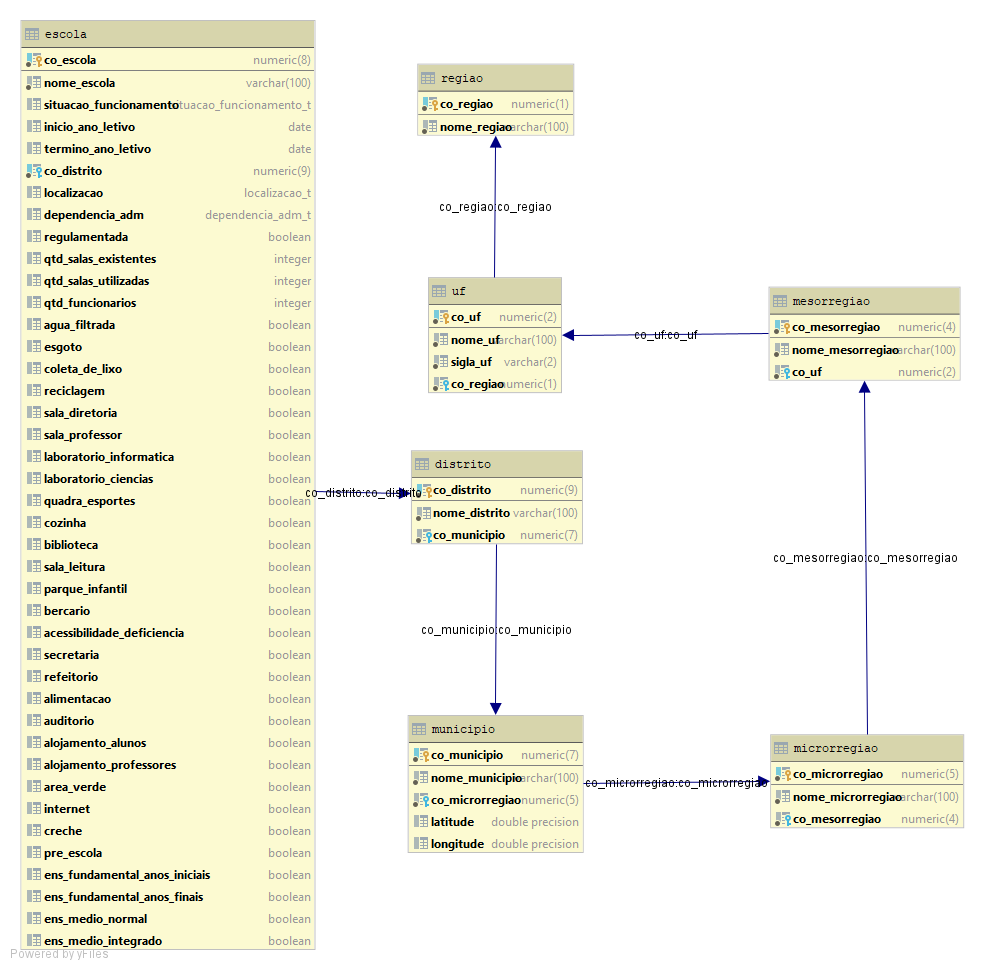
\includegraphics[scale=0.35]{diagrama_escolas_brasileiras.png}
    \caption{Diagrama do BD}
    \label{fig:diagrama}
\end{figure}

\pagebreak


\begin{flushleft}
    \textbf{Informações Básicas sobre a Escola}
\end{flushleft}

\begin{itemize}

    \item \texttt{co\_escola}: Código da Escola

    \item \texttt{nome\_escola}: Nome da Escola

    \item \texttt{situacao\_funcionamento}: Situação de Funcionamento da Escola (Em Atividade, Paralisada ou Extinta)

    \item \texttt{inicio\_ano\_letivo}: Data de Início do Ano Letivo

    \item \texttt{termino\_ano\_letivo}: Data de Término do Ano Letivo
    
    \item \texttt{dependencia\_adm}: Tipo de Dependência Administrativa da Escola (Federal, Estadual, Municipal ou Privada)

    \item \texttt{regulamentada}: Se a Escola é regulamentada ou não

    \item \texttt{qtd\_salas\_existentes}: Número de salas existentes na escola

    \item \texttt{qtd\_salas\_utilizadas}: Número de salas sendo efetivamente utilizadas na escola

    \item \texttt{qtd\_funcionarios}: Número de funcionários da escola

\end{itemize}

\begin{flushleft}
    \textbf{Informações de Localização Escola}
\end{flushleft}

\begin{itemize}

    \item \texttt{co\_distrito}: Código Completo do Distrito da Escola

    \item \texttt{localizacao}: Área da Localização da Escola (Urbana ou Rural)

\end{itemize}


    
\begin{flushleft}
    \textbf{Informações Adicionais sobre a Escola}
\end{flushleft}

\begin{itemize}

    \item \texttt{agua\_filtrada}: Se a Escola possui água filtrada ou não

    \item \texttt{esgoto}: Se a Escola possui sistema de esgoto ou não

    \item \texttt{coleta\_de\_lixo}: Se a Escola possui sistema de coleta de lixo ou não

    \item \texttt{reciclagem}: Se a Escola possui sistema de reciclagem de lixo ou não

\end{itemize}

\begin{flushleft}
    \textbf{Informações de Dependências da Escola}
\end{flushleft}

\begin{itemize}

    \item \texttt{sala\_diretoria}: Se a Escola possui uma sala de diretoria ou não

    \item \texttt{sala\_professor}: Se a Escola possui salas de professor ou não

    \item \texttt{laboratorio\_informatica}: Se a Escola possui um laboratório de informática ou não

    \item \texttt{laboratorio\_ciencias}: Se a Escola possui um laboratório de ciências ou não

    \item \texttt{quadra\_esportes}: Se a Escola possui quadra de esportes ou não

    \item \texttt{cozinha}: Se a Escola possui cozinha ou não

    \item \texttt{biblioteca}: Se a Escola possui biblioteca ou não

    \item \texttt{sala\_leitura}: Se a Escola possui sala de leitura ou não

    \item \texttt{parque\_infantil}: Se a Escola possui parque infantil ou não

    \item \texttt{bercario}: Se a Escola possui berçário ou não

    \item \texttt{acessibilidade\_deficiencia}: Se a Escola possui dependências e vias adequadas à alunos com deficiência ou mobilidade reduzida ou não
    
    \item \texttt{secretaria}: Se a Escola possui secretaria ou não

    \item \texttt{refeitorio}: Se a Escola possui refeitório ou não

    \item \texttt{alimentacao}: Se a Escola oferece alimentação ou não

    \item \texttt{auditorio}: Se a Escola possui auditório ou não

    \item \texttt{alojamento\_alunos}: Se a Escola possui alojamento para alunos ou não

    \item \texttt{alojamento\_professores}: Se a Escola possui alojamento para professores ou não

    \item \texttt{area\_verde}: Se a Escola possui uma área verde ou não

    \item \texttt{internet}: Se a Escola possui acesso à internet ou não

\end{itemize}

\begin{flushleft}
    \textbf{Informações de Oferta de Matrícula}
\end{flushleft}

\begin{itemize}

    \item \texttt{creche}: Se a Escola oferece creche ou não

    \item \texttt{pre\_escola}: Se a Escola oferece pré-escola ou não

    \item \texttt{ens\_fundamental\_anos\_iniciais}: Se a Escola oferece Ensino Fundamental do 1º ao 5º ano ou não

    \item \texttt{ens\_fundamental\_anos\_finais}: Se a Escola oferece Ensino Fundamental do 5º ao 9º ano ou não

    \item \texttt{ens\_medio\_normal}: Se a Escola oferece Ensino Médio do 1º ao 3º ano ou não

    \item \texttt{ens\_medio\_integrado}: Se a Escola oferece Ensino Médio integrado com Curso Técnico ou não

\end{itemize}

\section{Especificação de Consultas}

Nesta seção serão especificadas as consultas que farão parte do projeto. É importante ressaltar que são \textbf{duas} consultas, com atributos relativos (expressões regulares) e absolutos (expressões exatas). As consultas definidas pelo grupo serão apresentadas a seguir.

\begin{enumerate}
    \item 
        Buscar todas as escolas disponíveis em um determinado \texttt{Estado} (UF) e \texttt{Munícipio} (do Estado previamente selecionado), especificando um trecho do \texttt{nome da Escola} (dentre as previamente selecionadas no Munícipio). Além disso, o resultado obtido será ranqueado pelo \texttt{número de funcionários} da Escola.
        
        \textbf{Campos de busca}: \texttt{UF} e \texttt{Município} (absolutos), e \texttt{Nome da Escola} (relativo). 
        
        \textbf{Campos de visualização do resultado}: Inicialmente \texttt{código da escola}, \texttt{nome}, \texttt{situação de funcionamento}, \texttt{dependência administrativa} e  \texttt{ofertas de matricula}. Posteriormente, será possível a visualização dos demais campos da escola.
    
        \textbf{Operadores das condições}: \texttt{nome} da escola (\texttt{ILIKE}) e os demais (\texttt{=})
        
        \textbf{SQL}:
        \begin{Verbatim}[commandchars=\\\{\}]
SELECT  e.co\_escola, e.nome\_escola, e.situacao\_funcionamento,
            e.dependencia\_adm, e.bercario, e.creche, e.pre\_escola,
            e.ens\_fundamental\_anos\_iniciais, e.ens\_fundamental\_anos\_finais,
            e.ens\_medio\_normal, e.ens\_medio\_integrado
FROM escola e
JOIN distrito d on e.co\_distrito = d.co\_distrito
JOIN municipio m on d.co\_municipio = m.co\_municipio
JOIN microrregiao mi on m.co\_microrregiao = mi.co\_microrregiao
JOIN mesorregiao me on mi.co\_mesorregiao = me.co\_mesorregiao
JOIN uf u on me.co\_uf = u.co\_uf
WHERE u.co\_uf = \textcolor{MidnightBlue}{<codigo_uf>}
AND m.co\_municipio = \textcolor{MidnightBlue}{<codigo_municipio>}
AND e.nome\_escola ILIKE '\%\textcolor{MidnightBlue}{<nome_escola>}\%'
ORDER BY e.qtd\_funcionarios;
        \end{Verbatim}
    
    \vspace{0.5cm}
    \item 
        Buscar o número de escolas de uma região com cada tipo de situação de funcionamento, dependência administrativa e oferta de matrícula.
        
        \textbf{Campos de busca}: \texttt{Código da Região}.
        
        \textbf{Campos de visualização do resultado}: Quantidade de \texttt{Escolas} na \texttt{Região}, e desta região a quantidade de escolas \texttt{Em Atividade}, \texttt{Paralisada}, \texttt{Extinta}, \texttt{Federal}, \texttt{Estadual}, \texttt{Municipal}, \texttt{Privada} e com cada tipo de oferta de matrícula.
        
        \textbf{Operadores das condições}: \texttt{Código da Região} (\texttt{=}).
        
        \textbf{SQL}:
        \begin{Verbatim}[commandchars=\\\{\}]
SELECT
    GROUPING(e.bercario) g\_bercario, GROUPING(e.creche) g\_creche, 
    GROUPING(e.pre\_escola) g\_pe,
    GROUPING(e.ens\_fundamental\_anos\_iniciais) g\_efi,
    GROUPING(e.ens\_fundamental\_anos\_finais) g\_efii, 
    GROUPING(e.ens\_medio\_normal) g\_emn,
    GROUPING(e.ens\_medio\_integrado) g\_emi, 
    GROUPING(e.situacao\_funcionamento) g\_situacao,
    GROUPING(e.dependencia\_adm) g\_dep, 
    GROUPING(e.localizacao) g\_localizacao,
    e.bercario, e.creche, e.pre\_escola, e.ens\_fundamental\_anos\_iniciais,
    e.ens\_fundamental\_anos\_finais, e.ens\_medio\_normal,
    e.ens\_medio\_integrado,e.situacao\_funcionamento, e.dependencia\_adm, 
    e.localizacao, count(e.co\_escola) as qtd\_escolas
FROM escola e
JOIN distrito d on e.co\_distrito = d.co\_distrito
JOIN municipio m on d.co\_municipio = m.co\_municipio
JOIN microrregiao m2 on m.co\_microrregiao = m2.co\_microrregiao
JOIN mesorregiao m3 on m2.co\_mesorregiao = m3.co\_mesorregiao
JOIN uf u on m3.co\_uf = u.co\_uf
JOIN regiao r on u.co\_regiao = r.co\_regiao
WHERE r.co\_regiao = \textcolor{MidnightBlue}{<codigo_regiao>};
GROUP BY GROUPING SETS (
    (e.situacao\_funcionamento),
    (e.dependencia\_adm),
    (e.localizacao),
    (e.bercario),
    (e.creche),
    (e.pre\_escola),
    (e.ens\_fundamental\_anos\_iniciais),
    (e.ens\_fundamental\_anos\_finais),
    (e.ens\_medio\_normal),
    (e.ens\_medio\_integrado),
    ()
);
        \end{Verbatim}
        
\end{enumerate}


\section{Populando o BD}

Nesta seção será apresentado o modo como foi realizada a adição de dados ao banco de dados, bem como algumas informações técnicas de cada tabela. Vamos começar falando sobre de onde os dados foram retirados. Os dados do banco de escolas brasileiras foram retirados do \texttt{Microdados do INEP} do Censo Escolar 2018 (\url{http://inep.gov.br/microdados} . Como os dados vêm em uma tabela no excel, foi criado um script em PHP percorrendo a tabela e inserindo os dados no banco. Foram criados outros scripts também sobre outras tabelas auxiliares para a extração das informações dos \texttt{Distritos}, \texttt{Municípios}, \texttt{Microrregiões}, \texttt{Mesorregiões}, \texttt{Estados} e \texttt{Regiões}.

Quanto ao volume de dados final do banco, ou seja, o número de tuplas e o total em bytes de cada tabela, podemos visualizar na tabela abaixo:

\begin{table}[H]
  \centering
  \caption{Informações Tabelas}
    \begin{tabular}{|c|c|c|}
    \toprule
    \hline
    \textbf{Nome da Tabela} & \textbf{Nº de Tuplas} & \textbf{Tamanho} \\
    \midrule
    \hline
    \textbf{Escola} & 285975 & 58 MB \\
    \midrule
    \textbf{Distrito} & 10302 & 976 kB \\
    \midrule
    \textbf{Municipio} & 5570  & 744 kB \\
    \midrule
    \textbf{Microrregiao} & 558   & 88 kB \\
    \midrule
    \textbf{Mesorregiao} & 137   & 56 kB \\
    \midrule
    \textbf{Uf} & 27    & 24 kB \\
    \midrule
    \textbf{Regiao} & 5     & 24 kB \\
    \midrule
    \textbf{Total} & 302574 & 59,86 MB \\
    \bottomrule
    \hline
    \end{tabular}%
  \label{tab:addlabel}%
\end{table}%





\section{Otimização das Consultas}

Nesta seção iremos analisar o desempenho de cada uma das consultas especificadas na seção 3 (\texttt{Especificação das Consultas}). Utilizando técnicas de indexação e otimização, tentaremos alcançar um aumento significativo no desempenho das consultas.
O sistema de gerenciamento de banco de dados utilizado é o PostgreSQL, versão 9.5. A máquina utilizada para testes conta com um processador i7 e 8GB de memória RAM. As consultas foram executadas cinco vezes.

\subsection{Consulta 1 - Buscar Escolas Disponíveis}

Para fins de teste, utilizaremos os seguintes dados como parâmetros para realização das consultas: 
\begin{itemize}
    \item codigo\_uf = 35 (São Paulo)
    \item codigo\_municipio = 3552205 (Sorocaba)
    \item nome\_escola ILIKE '\%edu\%' (contém no nome o trecho 'edu')
\end{itemize}

\subsubsection{Operador JOIN}

Inicialmente executamos a consulta para obter o tempo de execução.

\vspace{0.5cm}

\begin{flushleft}
\textbf{CONSULTA SQL - JOIN}\\
\end{flushleft}

\begin{Verbatim}[commandchars=\\\{\}]
SELECT  e.co\_escola, e.nome\_escola, e.situacao\_funcionamento,
            e.dependencia\_adm, e.bercario, e.creche, e.pre\_escola,
            e.ens\_fundamental\_anos\_iniciais, e.ens\_fundamental\_anos\_finais,
            e.ens\_medio\_normal, e.ens\_medio\_integrado
FROM escola e
JOIN distrito d on e.co\_distrito = d.co\_distrito
JOIN municipio m on d.co\_municipio = m.co\_municipio
JOIN microrregiao mi on m.co\_microrregiao = mi.co\_microrregiao
JOIN mesorregiao me on mi.co\_mesorregiao = me.co\_mesorregiao
JOIN uf u on me.co\_uf = u.co\_uf
WHERE u.co\_uf = \textcolor{Red}{35}
AND m.co\_municipio = \textcolor{Red}{3552205}
AND e.nome\_escola ILIKE '\textcolor{Red}'
ORDER BY e.qtd\_funcionarios;
\end{Verbatim}

\begin{flushleft}
\textbf{TEMPO DE EXECUÇÃO}\\
\end{flushleft}
30 secs 246 msec.\\
96 rows affected.\\

Conforme o esperado, devido a muitos JOINs, o tempo da consulta foi ruim. Por conseguinte, executamos a mesma consulta com o comando \texttt{EXPLAIN ANALYZE}, obtendo o seguinte plano de execução:


% \vspace{0.5cm}
\begin{flushleft}
\textbf{PLANO DE EXECUÇÃO}\\
\end{flushleft}

\begin{figure}[H]
    \centering
    \includegraphics[width=\textwidth,height=\textwidth,keepaspectratio]{1-join.JPG}
    \caption{Consulta 1 - Original}
    \label{fig:diagrama}
\end{figure}

% EXPLICAÇÃO DO PLANO

Analisando o plano de execução, podemos observar que a \texttt{qtd\_funcionarios} proveniente da tabela \texttt{Escola} foi utilizada para ordenador os resultados obtidos e que o método de ordenação adotado foi o \texttt{quicksort} 


\subsubsection{Operador IN}

% EXPLICAÇÃO
A consulta inicial utiliza \texttt{JOIN}. Todavia, apesar de obtermos o resultado esperado, o tempo de execução foi consideravelmente alto. Uma medida adotada para obter o mesmo resultado, mas em um tempo de execução menor, foi utilizar \texttt{IN} ao invés de \texttt{JOIN}. 

\vspace{0.5cm}

\begin{flushleft}
\textbf{CONSULTA SQL - IN}\\
\end{flushleft}

\begin{Verbatim}[commandchars=\\\{\}]
SELECT  e.co\_escola, e.nome\_escola, e.situacao\_funcionamento, 
        e.dependencia\_adm, e.bercario, e.creche, e.pre\_escola,
        e.ens\_fundamental\_anos\_iniciais, e.ens\_fundamental\_anos\_finais,
        e.ens\_medio\_normal, e.ens\_medio\_integrado
FROM escola e
WHERE e.co\_distrito IN (
    SELECT d.co\_distrito
    FROM distrito d
    WHERE d.co\_municipio IN (
        SELECT m.co\_municipio
        FROM municipio m
        WHERE m.co\_microrregiao IN (
            SELECT mi.co\_microrregiao
            FROM microrregiao mi
            WHERE mi.co\_mesorregiao IN (
                SELECT me.co\_mesorregiao
                FROM mesorregiao me
                WHERE me.co\_uf = \textcolor{Red}{35}
            )
        )
    )
    AND d.co\_municipio = \textcolor{Red}{3552205}
)
AND e.nome\_escola ILIKE '\textcolor{Red}'
ORDER BY e.qtd\_funcionarios;
\end{Verbatim}

\begin{flushleft}
\textbf{TEMPO DE EXECUÇÃO}\\
\end{flushleft}
19 secs 94 msec.\\
96 rows affected.\\

\pagebreak
\begin{flushleft}
\textbf{PLANO DE EXECUÇÃO}\\
\end{flushleft}

\begin{figure}[H]
    \centering
    \includegraphics[width=\textwidth,height=\textheight,keepaspectratio]{1-in.JPG}
    \caption{Consulta 1 - Operador IN}
    \label{fig:diagrama}
\end{figure}

% EXPLICAÇÃO
É possível notar que ao adotarmos o \texttt{IN} no lugar de \texttt{JOIN} houve uma queda considerável de 11 secs 152 msec, aproximadamente 37\% do tempo inicial. 
\subsubsection{Criação do índice em nome escola}

Uma tentativa para melhorar o desempenho da consulta foi criar um índice para a coluna \texttt{nome\_escola} da tabela \texttt{Escola}:

\begin{verbatim}
    CREATE INDEX nome_escola_index
    ON escola(nome_escola)
    2 secs 936 msec.
\end{verbatim}

Realizamos novamente a mesma consulta com o operador \texttt{IN} e obtemos o seguinte tempo de execução:\\

16 secs 504 msec.

96 rows affected.\\

\pagebreak
\begin{flushleft}
\textbf{PLANO DE EXECUÇÃO}\\
\end{flushleft}

\begin{figure}[H]
    \centering
    \includegraphics[width=\textwidth,height=\textheight,keepaspectratio]{1-index.JPG}
    \caption{Consulta 1 - Criação do Índice \texttt{nome\_escola}}
    \label{fig:diagrama}
\end{figure}

Houve uma queda de aproximadamente 3 segundos em comparação com a consulta anterior, em que não havia o índice. Este valor representa uma diferença de aproximadamente 14\%.

Porém, podemos observar que mesmo com a criação do índice, este não foi utilizado. O otimizador de consultas do PostgreSQL achou melhor não utilizar o índice. Mesmo assim, podemos ver que ele modificou a ordem das operações e conseguiu uma queda de aproximadamente 3 segundos.

\subsubsection{Troca de ILIKE por LIKE}

A última técnica de  otimização utilizada foi trocar o operador \texttt{ILIKE} pelo operador \texttt{LIKE}. O operador \texttt{ILIKE} não considera letras maiúsculas e minúsculas, fato que faz com que haja um aumento no tempo de execução da consulta. 

\vspace{0.5cm}
\begin{flushleft}
\textbf{CONSULTA SQL - LIKE}\\
\end{flushleft}

\begin{Verbatim}[commandchars=\\\{\}]
SELECT  e.co\_escola, e.nome\_escola, e.situacao\_funcionamento, 
        e.dependencia\_adm, e.bercario, e.creche, e.pre\_escola,
        e.ens\_fundamental\_anos\_iniciais, e.ens\_fundamental\_anos\_finais,
        e.ens\_medio\_normal, e.ens\_medio\_integrado
FROM escola e
WHERE e.co\_distrito IN (
    SELECT d.co\_distrito
    FROM distrito d
    WHERE d.co\_municipio IN (
        SELECT m.co\_municipio
        FROM municipio m
        WHERE m.co\_microrregiao IN (
            SELECT mi.co\_microrregiao
            FROM microrregiao mi
            WHERE mi.co\_mesorregiao IN (
                SELECT me.co\_mesorregiao
                FROM mesorregiao me
                WHERE me.co\_uf = \textcolor{Red}{35}
            )
        )
    )
    AND d.co\_municipio = \textcolor{Red}{3552205}
)
AND e.nome\_escola LIKE \textcolor{Red}{'%EDU%'}
ORDER BY e.qtd\_funcionarios;
\end{Verbatim}

\begin{flushleft}
\textbf{TEMPO DE EXECUÇÃO}\\
\end{flushleft}
2 secs 8 msec.\\
96 rows affected.\\




\begin{flushleft}
\textbf{PLANO DE EXECUÇÃO}\\
\end{flushleft}

\begin{figure}[H]
    \centering
    \includegraphics[width=\textwidth,height=\textwidth,keepaspectratio]{1-like.JPG}
    \caption{Consulta 1 - Operador LIKE}
    \label{fig:diagrama}
\end{figure}

Podemos notar que ao realizarmos a mudança dos operadores, houve uma queda aproximadamente 14 segundos em relação ao tempo de execução da consulta anterior. Este tempo representa um diferença de aproximadamente 87\%.   

Apesar do plano de execução dos operadores serem iguais, como o operador \texttt{LIKE} leva em consideração letras minúsculas e maiúsculas, o otimizador conseguiu realizar a consulta muito mais rapidamente.

%-----------------

\subsubsection{Materialized Views}

Outra tentativa de otimização foi realizar a criação de views materializadas, ou seja, que ficam em armazenadas em disco. Deste modo, uma \texttt{MATERIALIZED VIEW} foi criada para cada \texttt{estado} da tabela \texttt{Estado}. 

Para conseguir fazer isto, foi criado um script na linguagem PHP para criar, para cada estado, uma view contendo os códigos dos distritos daquele estado. Foi dado o nome \texttt{distrito<codigo\_estado>}.

Criadas as views, basta realizarmos uma seleção dos códigos dos distritos presentes na view específica do estado desejado, não precisando mais percorrer todos os IN's da consulta anterior.

\vspace{0.5cm}
\begin{flushleft}
\textbf{CONSULTA SQL - COM MATERIALIZED VIEW}\\
\end{flushleft}

\begin{Verbatim}[commandchars=\\\{\}]
SELECT  e.co\_escola, e.nome\_escola, e.situacao\_funcionamento, 
        e.dependencia\_adm, e.bercario, e.creche, e.pre\_escola,
        e.ens\_fundamental\_anos\_iniciais, e.ens\_fundamental\_anos\_finais,
        e.ens\_medio\_normal, e.ens\_medio\_integrado
FROM escola e
WHERE e.co\_distrito in (
    SELECT co\_distrito
    FROM distritos\textcolor{Red}{35} d
    WHERE d.co\_municipio = \textcolor{Red}{3552205}
)
AND e.nome\_escola LIKE \textcolor{Red}{'%EDU%'}
ORDER BY e.qtd\_funcionarios;
\end{Verbatim}

\vspace{0.01cm}
\begin{flushleft}
\textbf{TEMPO DE EXECUÇÃO}\\
\end{flushleft}
1 secs 613 msec.\\

\begin{flushleft}
\textbf{PLANO DE EXECUÇÃO}\\
\end{flushleft}

\begin{figure}[H]
    \centering
    \includegraphics[width=\textwidth,height=\textwidth,keepaspectratio]{1-view.JPG}
    \caption{Consulta 1 - com MATERIALIZED VIEW}
    \label{fig:diagrama}
\end{figure}

Podemos observar que o tempo de execução caiu, porém não significativamente, apenas 395ms. Pelo plano de consulta podemos verificar que o otimizador realizou uma busca sequencial no código do distrito na view de distritos e comparou com o código do distrito na tabela escola. Por fim, realizou uma ordenação com quicksort pela quantidade de funcionários.


\subsubsection{Criação do Índice em Escola(Código Distrito)}

A última otimização realizada foi a criação de um índice na coluna \texttt{co\_distrito} da tabela \texttt{Escola}. A SQL utilizada para a criação do índice e o tempo de execução podem ser observados a seguir:

\vspace{0.25cm}
\begin{verbatim}
    CREATE INDEX e_co_distrito_index 
    ON escola(co_distrito)
    3 secs 607 msec.
\end{verbatim}
\vspace{0.25cm}

Realizando novamente a mesma consulta do item anterior, observamos os seguintes resultados:

\vspace{0.01cm}
\begin{flushleft}
\textbf{TEMPO DE EXECUÇÃO}\\
\end{flushleft}
482 msec.\\

\begin{flushleft}
\textbf{PLANO DE EXECUÇÃO}\\
\end{flushleft}

\begin{figure}[H]
    \centering
    \includegraphics[width=\textwidth,height=\textwidth,keepaspectratio]{1-index-co-distrito.JPG}
    \caption{Consulta 1 - com Índice no Código do Distrito}
    \label{fig:diagrama}
\end{figure}

Como podemos observar, o tempo de execução caiu para apenas 482 ms! Uma diminuição de 70\% do valor anterior, que ainda não continha o índice. Fica clara esta diferença ao visualizar o plano de execução, uma vez que o otimizador utilizou o novo índice criado.


\subsubsection{Conclusão - Consulta 1}
\vspace{0.5cm}
Na Tabela 1 podemos observar as diferenças, em porcentagem, dos tempos de execução de cada um dos testes realizados para a Consulta 1, e observar que conseguimos uma melhora final de 98,4\% em relação ao tempo inicial:

\begin{table}[htbp]
  \centering
  \caption{Comparação Consulta 1}
    \resizebox{\textwidth}{!}{\begin{tabular}{|l|c|c|c|}
    \hline
    \toprule
    \textbf{Testes} & \textbf{Tempo (ms)} & \textbf{Diferença com Anterior (\%)} & \multicolumn{1}{l|}{\textbf{Diferença com Original (\%)}} \\
    \hline
    \midrule
    Consulta Inicial (JOIN) & 30246 & -     & - \\
    \midrule
    IN    & 19094 & 36,87 & 36,87 \\
    \midrule
    ÍNDICE & 16504 & 13,56 & 45,43 \\
    \midrule
    LIKE  & 2008  & 87,83 & 93,36 \\
    \midrule
    MATERIALIZED VIEW & 1613  & 19,67 & 94,66 \\
    \midrule
    ÍNDICE (co\_distrito) & 482   & 70,11 & 98,4 \\
    \bottomrule
    \hline
    \end{tabular}}%
  \label{tab:compconsulta1}%
\end{table}%


\subsection{Consulta 2 - Quantidade de Escolas de cada Dependência Administrativa}

A segunda consulta também foi inicialmente realizada com o operador \texttt{JOIN}. Nesta consulta foi utilizada a cláusula \texttt{GROUP BY GROUPING SETS}, a qual realiza o agrupamento dos resultados de acordo com o específicado (no caso por situação de funcionamento, dependência administrativa e cada tipo de oferta de matrícula). O parênteses vazio na última linha do \texttt{GROUPING SETS} serve para recuperar o total de escolas. Para fins de teste, utilizaremos o seguinte dado como parâmetro para realização das consultas: 
\begin{itemize}
    \item codigo\_regiao = 3 (Sudeste)
\end{itemize}

\subsubsection{Operador JOIN}

O primeiro teste foi realizado com o operador \texttt{JOIN}.

\vspace{0.5cm}
\begin{flushleft}
\textbf{CONSULTA SQL - JOIN}\\
\end{flushleft}

\begin{Verbatim}[commandchars=\\\{\}]
SELECT
    GROUPING(e.bercario) g\_bercario, GROUPING(e.creche) g\_creche, 
    GROUPING(e.pre\_escola) g\_pe,
    GROUPING(e.ens\_fundamental\_anos\_iniciais) g\_efi,
    GROUPING(e.ens\_fundamental\_anos\_finais) g\_efii, 
    GROUPING(e.ens\_medio\_normal) g\_emn,
    GROUPING(e.ens\_medio\_integrado) g\_emi, 
    GROUPING(e.situacao\_funcionamento) g\_situacao,
    GROUPING(e.dependencia\_adm) g\_dep, 
    GROUPING(e.localizacao) g\_localizacao,
    e.bercario, e.creche, e.pre\_escola, e.ens\_fundamental\_anos\_iniciais,
    e.ens\_fundamental\_anos\_finais, e.ens\_medio\_normal,
    e.ens\_medio\_integrado,e.situacao\_funcionamento, e.dependencia\_adm, 
    e.localizacao, count(e.co\_escola) as qtd\_escolas
FROM escola e
JOIN distrito d on e.co\_distrito = d.co\_distrito
JOIN municipio m on d.co\_municipio = m.co\_municipio
JOIN microrregiao m2 on m.co\_microrregiao = m2.co\_microrregiao
JOIN mesorregiao m3 on m2.co\_mesorregiao = m3.co\_mesorregiao
JOIN uf u on m3.co\_uf = u.co\_uf
JOIN regiao r on u.co\_regiao = r.co\_regiao
WHERE r.co\_regiao = \textcolor{Red}{3};
GROUP BY GROUPING SETS (
    (e.situacao\_funcionamento),
    (e.dependencia\_adm),
    (e.localizacao),
    (e.bercario),
    (e.creche),
    (e.pre\_escola),
    (e.ens\_fundamental\_anos\_iniciais),
    (e.ens\_fundamental\_anos\_finais),
    (e.ens\_medio\_normal),
    (e.ens\_medio\_integrado),
    ()
);
\end{Verbatim}

\begin{flushleft}
\textbf{TEMPO DE EXECUÇÃO}\\
\end{flushleft}
4 secs 206 msec.\\

\begin{flushleft}
\textbf{PLANO DE EXECUÇÃO}\\
\end{flushleft}

\begin{figure}[H]
    \centering
    \includegraphics[width=\textwidth,height=\textwidth,keepaspectratio]{2-join.JPG}
    \caption{Consulta 2 - Original}
    \label{fig:diagrama}
\end{figure}

Podemos observar no plano de execução que o índice criado no código do \texttt{Distrito} (\texttt{e\_co\_distrito\_index} para otimizar a consulta um, também foi utilizado por esta consulta. Logo, este índice também foi responsável pelo baixo tempo de execução inicial desta consulta.

\subsubsection{Operador IN}

Com intuíto de diminuir o tempo de execução modificamos a consulta para a utilizarmos o operador \texttt{IN} ao invés do operador \texttt{JOIN}.

\vspace{0.5cm}

\begin{flushleft}
\textbf{CONSULTA SQL - IN}\\
\end{flushleft}

\begin{Verbatim}[commandchars=\\\{\}]
SELECT
    GROUPING(e.bercario) g\_bercario, GROUPING(e.creche) g\_creche, 
    GROUPING(e.pre\_escola) g\_pe,
    GROUPING(e.ens\_fundamental\_anos\_iniciais) g\_efi,
    GROUPING(e.ens\_fundamental\_anos\_finais) g\_efii, 
    GROUPING(e.ens\_medio\_normal) g\_emn,
    GROUPING(e.ens\_medio\_integrado) g\_emi, 
    GROUPING(e.situacao\_funcionamento) g\_situacao,
    GROUPING(e.dependencia\_adm) g\_dep, 
    GROUPING(e.localizacao) g\_localizacao,
    e.bercario, e.creche, e.pre\_escola, e.ens\_fundamental\_anos\_iniciais,
    e.ens\_fundamental\_anos\_finais, e.ens\_medio\_normal,
    e.ens\_medio\_integrado,e.situacao\_funcionamento, e.dependencia\_adm, 
    e.localizacao, count(e.co\_escola) as qtd\_escolas
FROM escola e
WHERE e.co\_distrito IN (
    SELECT d.co\_distrito
    FROM distrito d
    WHERE d.co\_municipio IN (
        SELECT m.co\_municipio
        FROM municipio m
        WHERE m.co\_microrregiao IN (
            SELECT mi.co\_microrregiao
            FROM microrregiao mi
            WHERE mi.co\_mesorregiao IN (
                SELECT me.co\_mesorregiao
                FROM mesorregiao me
                WHERE me.co\_uf IN (
                    SELECT u.co\_uf
                    FROM uf u
                    WHERE u.co\_regiao = \textcolor{Red}{3};
                )
            )
        )
    )
)
GROUP BY GROUPING SETS (
    (e.situacao\_funcionamento),
    (e.dependencia\_adm),
    (e.localizacao),
    (e.bercario),
    (e.creche),
    (e.pre\_escola),
    (e.ens\_fundamental\_anos\_iniciais),
    (e.ens\_fundamental\_anos\_finais),
    (e.ens\_medio\_normal),
    (e.ens\_medio\_integrado),
    ()
);
\end{Verbatim}

\begin{flushleft}
\textbf{TEMPO DE EXECUÇÃO}\\
\end{flushleft}
2 secs 476 msec.\\

\begin{flushleft}
\textbf{PLANO DE EXECUÇÃO}\\
\end{flushleft}

\begin{figure}[H]
    \centering
    \includegraphics[width=\textwidth,height=\textwidth,keepaspectratio]{2-in.JPG}
    \caption{Consulta 2 - Operador IN}
    \label{fig:diagrama}
\end{figure}

Podemos observar que o tempo de execução sofreu uma redução de 1 sec 730 msec. Queda significava se observarmos que este valor representa uma redução de aproximadamente 41\% em relação ao tempo anterior.

%---------------------------------

\subsubsection{Materialized View}

Observamos que a criação de views com os códigos dos distritos de cada estado foram responsáveis por uma melhoria significativa no tempo de execução da consulta 1. Logo, a última otimização realizada para a segunda consulta foi a criação de \texttt{Materialized Views} contendo os distritos (código e nome do distrito, além do código de seu município) de cada região. O intuito desta alteração foi reduzir ainda mais o tempo da consulta, mesmo que já pequeno, visto que para a aplicação quanto mais rápido melhor.

\vspace{0.5cm}

\begin{flushleft}
\textbf{CONSULTA SQL - View}\\
\end{flushleft}

\begin{Verbatim}[commandchars=\\\{\}]
SELECT
SELECT
    GROUPING(e.bercario) g\_bercario, GROUPING(e.creche) g\_creche, 
    GROUPING(e.pre\_escola) g\_pe,
    GROUPING(e.ens\_fundamental\_anos\_iniciais) g\_efi,
    GROUPING(e.ens\_fundamental\_anos\_finais) g\_efii, 
    GROUPING(e.ens\_medio\_normal) g\_emn,
    GROUPING(e.ens\_medio\_integrado) g\_emi, 
    GROUPING(e.situacao\_funcionamento) g\_situacao,
    GROUPING(e.dependencia\_adm) g\_dep, 
    GROUPING(e.localizacao) g\_localizacao,
    e.bercario, e.creche, e.pre\_escola, e.ens\_fundamental\_anos\_iniciais,
    e.ens\_fundamental\_anos\_finais, e.ens\_medio\_normal,
    e.ens\_medio\_integrado,e.situacao\_funcionamento, e.dependencia\_adm, 
    e.localizacao, count(e.co\_escola) as qtd\_escolas
FROM escola e
WHERE e.co\_distrito IN (
    SELECT d.co\_distrito
    FROM distritos\_regiao3 d
)
GROUP BY GROUPING SETS (
    (e.situacao\_funcionamento),
    (e.dependencia\_adm),
    (e.localizacao),
    (e.bercario),
    (e.creche),
    (e.pre\_escola),
    (e.ens\_fundamental\_anos\_iniciais),
    (e.ens\_fundamental\_anos\_finais),
    (e.ens\_medio\_normal),
    (e.ens\_medio\_integrado),
    ()
);
\end{Verbatim}

\begin{flushleft}
\textbf{TEMPO DE EXECUÇÃO}\\
\end{flushleft}
1 secs 644 msec.\\

\begin{flushleft}
\textbf{PLANO DE EXECUÇÃO}\\
\end{flushleft}

\begin{figure}[H]
    \centering
    \includegraphics[width=\textwidth,height=\textwidth,keepaspectratio]{2-view.JPG}
    \caption{Consulta 2 - View}
    \label{fig:diagrama}
\end{figure}

Podemos observar pelo plano de execução que este ficou bem mais simples em relação aos outros, visto que agora bastou uma busca sequencial na view da região especificada, sem ter que realizar todos os joins com as outras tabelas.

\subsubsection{Conclusão - Consulta 2}

Com as otimizações realizadas, conseguimos uma melhora total de 60,91\% no tempo de execução da consulta. Na Tabela 2 podemos observar as comparações entre os tempos de execução de cada um dos testes realizados para a consulta 2:

\begin{table}[htbp]
  \centering
  \caption{Comparação - Consulta 2}
    \resizebox{\textwidth}{!}{\begin{tabular}{|l|c|c|c|}
    \toprule
    \hline
    \textbf{Testes} & \textbf{Tempo (ms)} & \textbf{Diferença com Anterior (\%)} & \multicolumn{1}{l|}{\textbf{Diferença com Original (\%)}} \\
    \midrule
    \hline
    Consulta Inicial (JOIN) & 4206  & -     & - \\
    \midrule
    IN    & 2476  & 41,13 & 41,13 \\
    \midrule
    MATERIALIZED VIEW & 1644  & 33,6  & 60,91 \\
    \bottomrule
    \hline
    \end{tabular}}%
  \label{tab:addlabel}%
\end{table}%


\section{Segurança e Controle de Acesso}

Nesta seção iremos mostrar e analisar as técnicas utilizadas no banco para segurança e controle de acesso aos dados. Iremos citar as técnicas utilizadas para prevenção de SQL Injection e os usuários criados para o controle das operações permitidas sobre o banco das escolas.

\subsection{Prevenção de SQL Injection}

Para a prevenção de SQL Injection, foram utilizadas basicamente duas técnicas: a utilização de \texttt{stored procedures} e de \texttt{prepared statements} para tratamento das consultas SQL.

\begin{flushleft}
\textbf{PROCEDURES}\\
\end{flushleft}



\begin{flushleft}
\textbf{PREPARED STATEMENT}\\
\end{flushleft}


\subsection{Usuários para Controle de Acesso}

Foram criados três usuários para realizar o controle de acesso ao bando de dados. Os usuários criados foram:

\begin{itemize}
    \item \texttt{admin}
    \item \texttt{gerente}
    \item \texttt{diretor}
    \item \texttt{cliente}
\end{itemize}

O \texttt{admin} possui todos os privilégios, ou seja, os privilégios de seleção, inserção, atualização e dele.ão sobre todas as tabelas d Abancolém disso, foi çespecifio cado o privilégio \texttt{CREATEROLE}, assim o \texttt{admin} pode criar outros usuários. Também foi especificado \texttt{GRANT OPTION}, deste modo, ele recebe o privilégio de conceder privilégios a outros usuários.

À partir do \texttt{admin} foram criados os usuários \texttt{gerente}, \texttt{diretor} e \texttt{cliente}. Ao gerente foram dados os privilégios de seleção e atualização sobre todas as tabelas. Ao \texttt{diretor} foram concedidos os privilégios de seleção e inserção sobre todas as tabelas.

Por fim, ao \texttt{cliente} foi apenas dado o privilégio de seleção sobre as tabelas. É importante ressaltar que a todos os três usuários criados foi especificada a opção \texttt{NOINHERIT}, ou seja, não herdam nenhum dos privilégios de cima.

Para melhor visualizar os usuários criados, bem como cada privilégio concedido a cada um, podemos observar a tabela abaixo:

\begin{table}[htbp]
  \centering
  \caption{Privilégios Usuários}
    \begin{tabular}{|l|l|l|l|l|}
    \toprule
    \hline
          & \textbf{admin} & \textbf{diretor} & \textbf{gerente} & \textbf{cliente} \\
    \midrule
    \hline
    \textbf{escola} & S,I,U,D & S,I   & S,U   & S \\
    \midrule
    \textbf{distrito} & S,I,U,D & S,I   & S,U   & S \\
    \midrule
    \textbf{municipio} & S,I,U,D & S,I   & S,U   & S \\
    \midrule
    \textbf{microrregiao} & S,I,U,D & S,I   & S,U   & S \\
    \midrule
    \textbf{mesorregiao} & S,I,U,D & S,I   & S,U   & S \\
    \midrule
    \textbf{uf} & S,I,U,D & S,I   & S,U   & S \\
    \midrule
    \textbf{regiao} & S,I,U,D & S,I   & S,U   & S \\
    \bottomrule
    \hline
    \end{tabular}%
  \label{tab:addlabel}%
\end{table}%

Além disso, foi criado também o diagrama de concessões, que nos permite visualizar melhor ainda os privilégios de cada usuário, bem como quem os concedeu:

\begin{figure}[H]
    \centering
    \includegraphics[scale=0.3]{arvore-privilegios.JPG}
    \caption{Diagrama de Concessões}
    \label{fig:diagrama}
\end{figure}



\end{document}